\documentclass[a4paper,10pt,landscape]{article}
\usepackage[margin=0.6cm]{geometry}
\usepackage[T1]{fontenc}
\usepackage[utf8]{inputenc}
\usepackage{xcolor}
\usepackage{tikz}
\usetikzlibrary{arrows.meta,positioning,calc,shapes.geometric}
\pagestyle{empty}
\setlength{\parindent}{0pt}
\renewcommand{\familydefault}{\sfdefault}

\definecolor{zw}{RGB}{0,0,0}
\definecolor{bl}{RGB}{20,70,180}
\definecolor{gr}{RGB}{20,120,40}
\definecolor{ro}{RGB}{180,20,20}

\newcommand{\ZW}[1]{\textcolor{zw}{#1}}
\newcommand{\BL}[1]{\textcolor{bl}{#1}}
\newcommand{\GR}[1]{\textcolor{gr}{#1}}
\newcommand{\RO}[1]{\textcolor{ro}{#1}}

\begin{document}

% ========================= LES 1 =========================
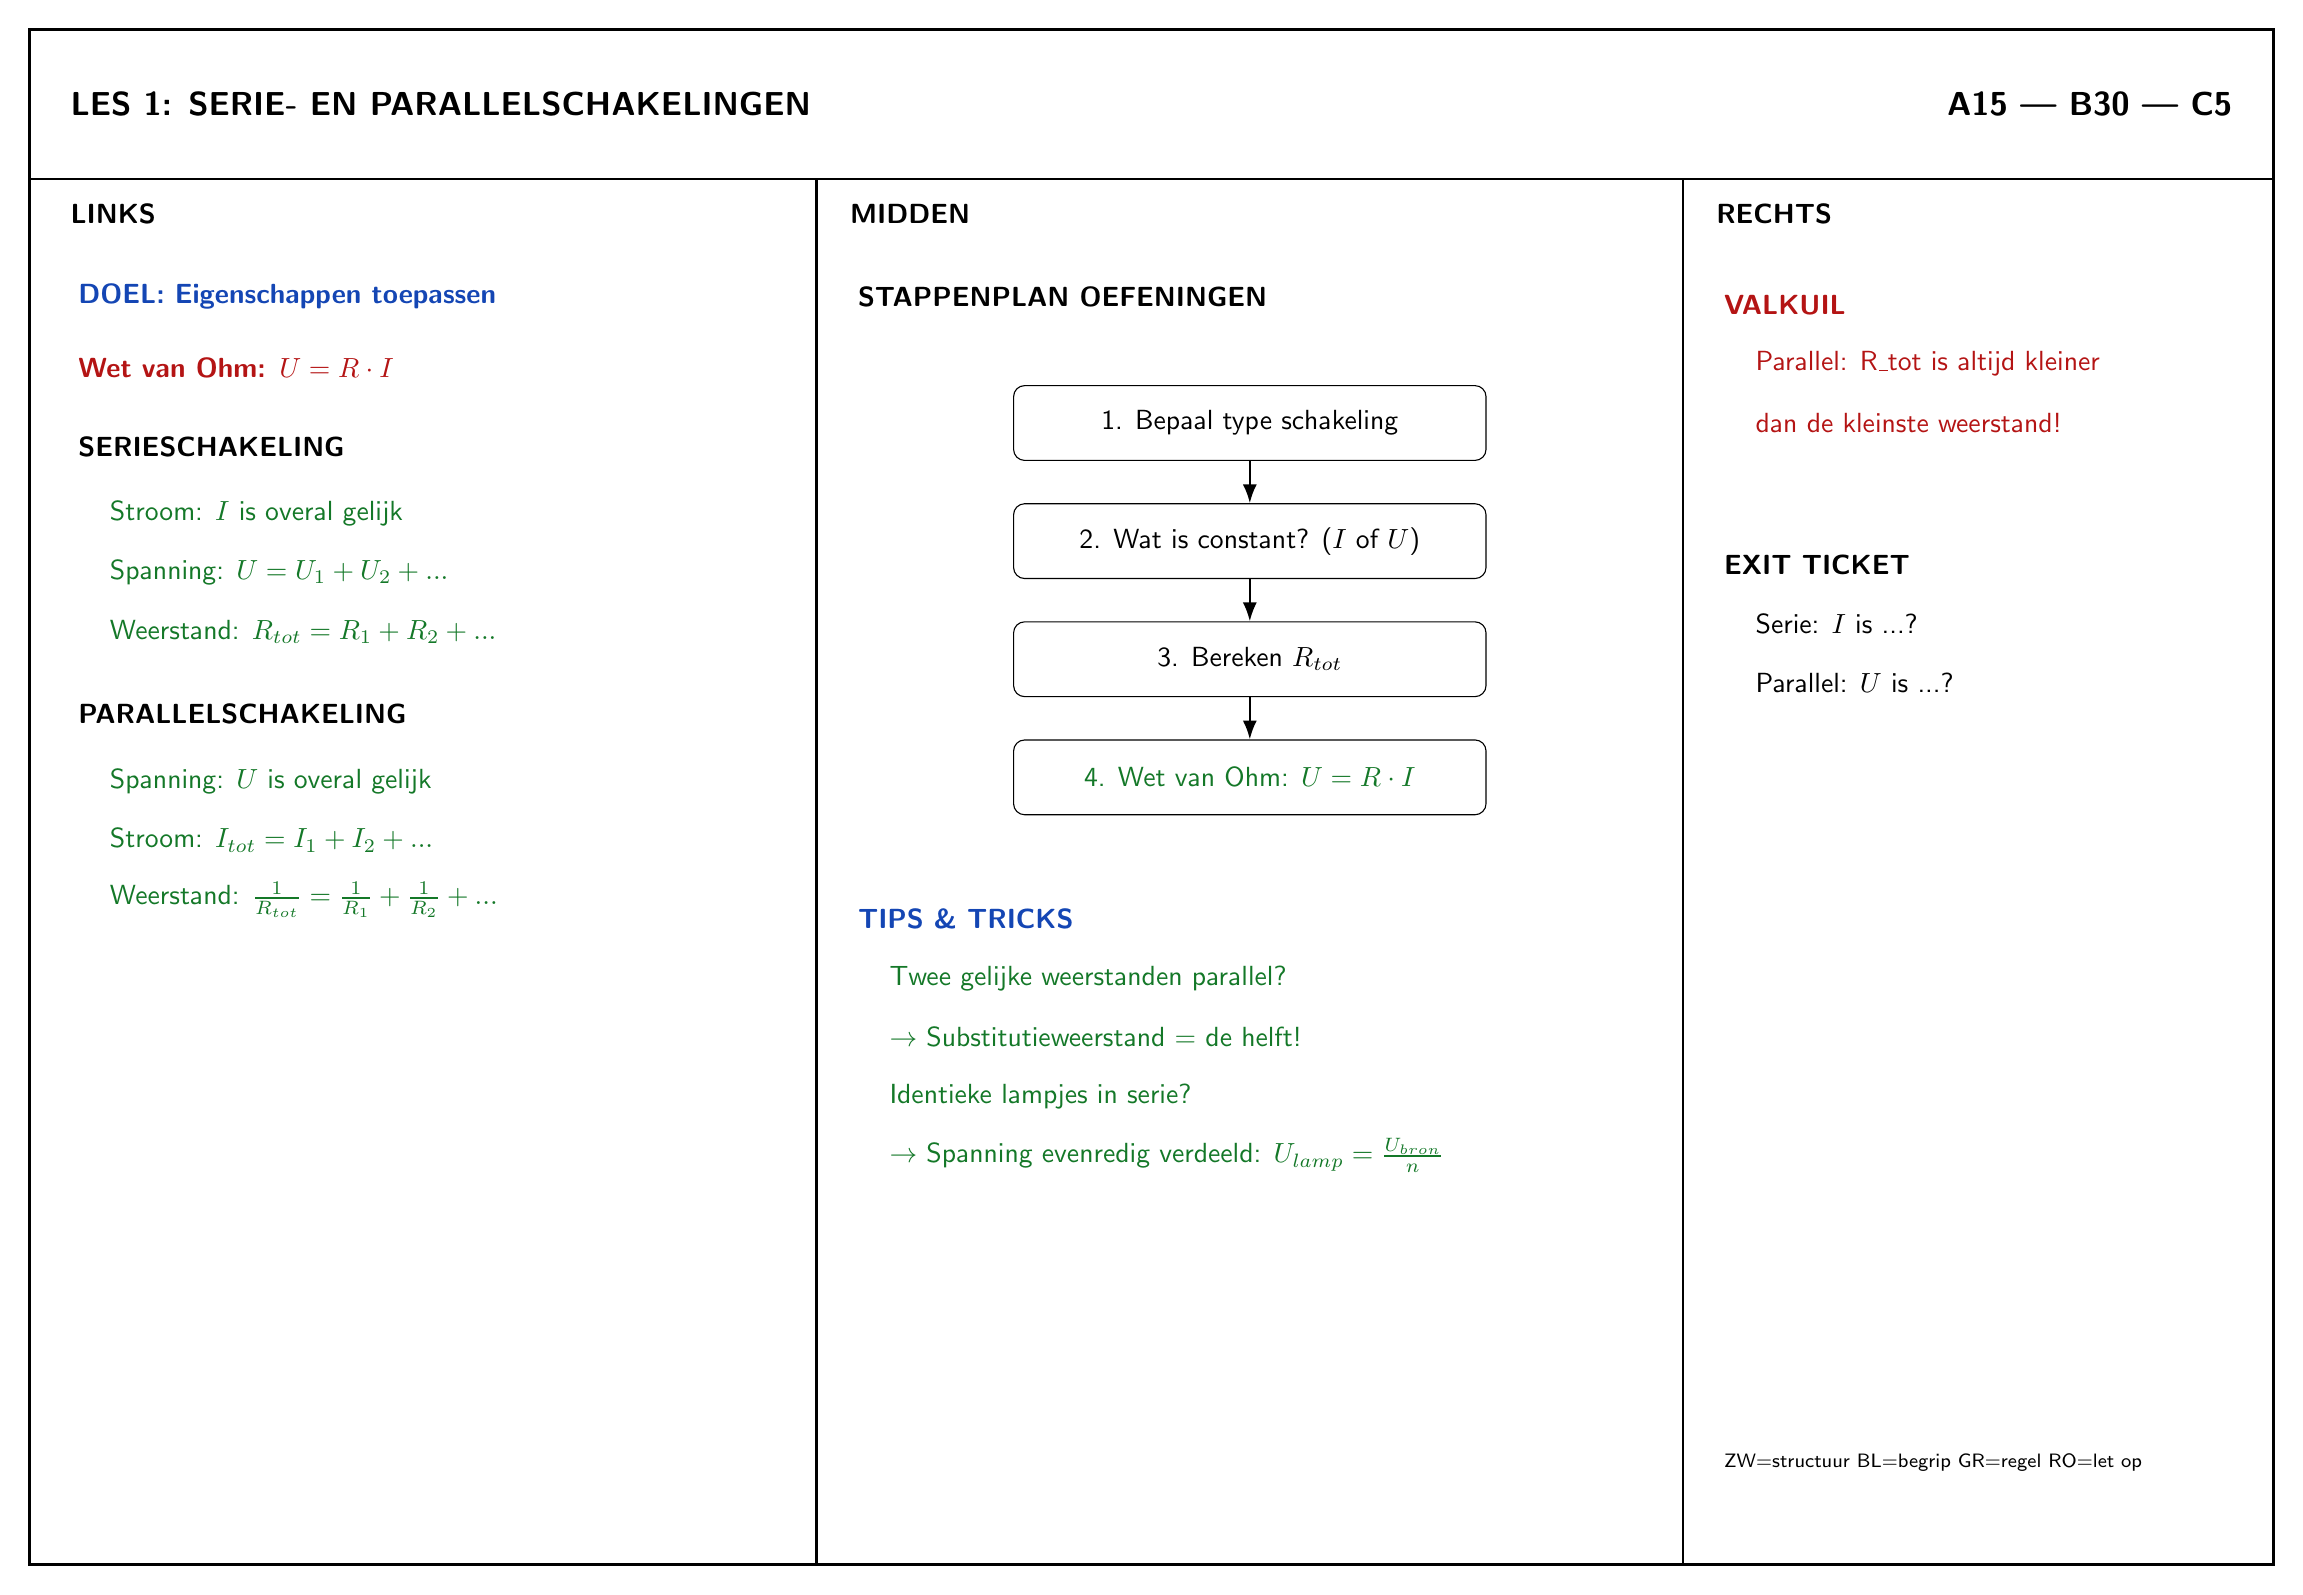
\begin{tikzpicture}[x=1cm,y=1cm]
  % outer board
  \draw[line width=1.2pt] (0,0) rectangle (28.5,19.5);

  % top bar
  \draw[line width=0.9pt] (0,17.6) -- (28.5,17.6);
  \node[anchor=west,font=\bfseries\large] at (0.4,18.55) {\ZW{LES 1: SERIE- EN PARALLELSCHAKELINGEN}};
  \node[anchor=east,font=\bfseries\large] at (28.1,18.55) {\ZW{A15 | B30 | C5}};

  % vertical columns
  \draw[line width=0.9pt] (10.0,0) -- (10.0,17.6);
  \draw[line width=0.9pt] (21.0,0) -- (21.0,17.6);

  % column titles
  \node[anchor=west,font=\bfseries] at (0.4,17.15) {\ZW{LINKS}};
  \node[anchor=west,font=\bfseries] at (10.3,17.15) {\ZW{MIDDEN}};
  \node[anchor=west,font=\bfseries] at (21.3,17.15) {\ZW{RECHTS}};

  % left content
  \node[anchor=west,font=\bfseries] at (0.5,16.1) {\BL{DOEL: Eigenschappen toepassen}};
  \node[anchor=west,font=\bfseries] at (0.5,15.2) {\RO{Wet van Ohm: $U = R \cdot I$}};
  
  \node[anchor=west,font=\bfseries] at (0.5,14.2) {\ZW{SERIESCHAKELING}};
  \node[anchor=west] at (0.9,13.35) {\GR{Stroom: $I$ is overal gelijk}};
  \node[anchor=west] at (0.9,12.6) {\GR{Spanning: $U = U_1 + U_2 + ...$}};
  \node[anchor=west] at (0.9,11.85) {\GR{Weerstand: $R_{tot} = R_1 + R_2 + ...$}};

  \node[anchor=west,font=\bfseries] at (0.5,10.8) {\ZW{PARALLELSCHAKELING}};
  \node[anchor=west] at (0.9,9.95) {\GR{Spanning: $U$ is overal gelijk}};
  \node[anchor=west] at (0.9,9.2) {\GR{Stroom: $I_{tot} = I_1 + I_2 + ...$}};
  \node[anchor=west] at (0.9,8.45) {\GR{Weerstand: $\frac{1}{R_{tot}} = \frac{1}{R_1} + \frac{1}{R_2} + ...$}};

  % middle content
  \node[anchor=west,font=\bfseries] at (10.4,16.1) {\ZW{STAPPENPLAN OEFENINGEN}};
  \node[draw,rounded corners,minimum width=6.0cm,minimum height=0.95cm,align=center] (s1) at (15.5,14.5) {\ZW{1. Bepaal type schakeling}};
  \node[draw,rounded corners,minimum width=6.0cm,minimum height=0.95cm,align=center] (s2) at (15.5,13.0) {\ZW{2. Wat is constant? ($I$ of $U$)}};
  \node[draw,rounded corners,minimum width=6.0cm,minimum height=0.95cm,align=center] (s3) at (15.5,11.5) {\ZW{3. Bereken $R_{tot}$}};
  \node[draw,rounded corners,minimum width=6.0cm,minimum height=0.95cm,align=center] (s4) at (15.5,10.0) {\GR{4. Wet van Ohm: $U = R \cdot I$}};

  \draw[-{Latex[length=2.4mm]},line width=0.8pt] (s1) -- (s2);
  \draw[-{Latex[length=2.4mm]},line width=0.8pt] (s2) -- (s3);
  \draw[-{Latex[length=2.4mm]},line width=0.8pt] (s3) -- (s4);

  \node[anchor=west,font=\bfseries] at (10.4,8.2) {\BL{TIPS \& TRICKS}};
  \node[anchor=west] at (10.8,7.45) {\GR{Twee gelijke weerstanden parallel?}};
  \node[anchor=west] at (10.8,6.7) {\GR{$\rightarrow$ Substitutieweerstand = de helft!}};
  \node[anchor=west] at (10.8,5.95) {\GR{Identieke lampjes in serie?}};
  \node[anchor=west] at (10.8,5.2) {\GR{$\rightarrow$ Spanning evenredig verdeeld: $U_{lamp} = \frac{U_{bron}}{n}$}};

  % right content
  \node[anchor=west,font=\bfseries] at (21.4,16.0) {\RO{VALKUIL}};
  \node[anchor=west] at (21.8,15.25) {\RO{Parallel: R\_tot is altijd kleiner}};
  \node[anchor=west] at (21.8,14.5) {\RO{dan de kleinste weerstand!}};

  \node[anchor=west,font=\bfseries] at (21.4,12.7) {\ZW{EXIT TICKET}};
  \node[anchor=west] at (21.8,11.95) {\ZW{Serie: $I$ is ...?}};
  \node[anchor=west] at (21.8,11.2) {\ZW{Parallel: $U$ is ...?}};

  % marker legend
  \node[anchor=west,font=\scriptsize] at (21.4,1.3) {\ZW{ZW=structuur  BL=begrip  GR=regel  RO=let op}};
\end{tikzpicture}

\newpage

% ========================= LES 2 =========================
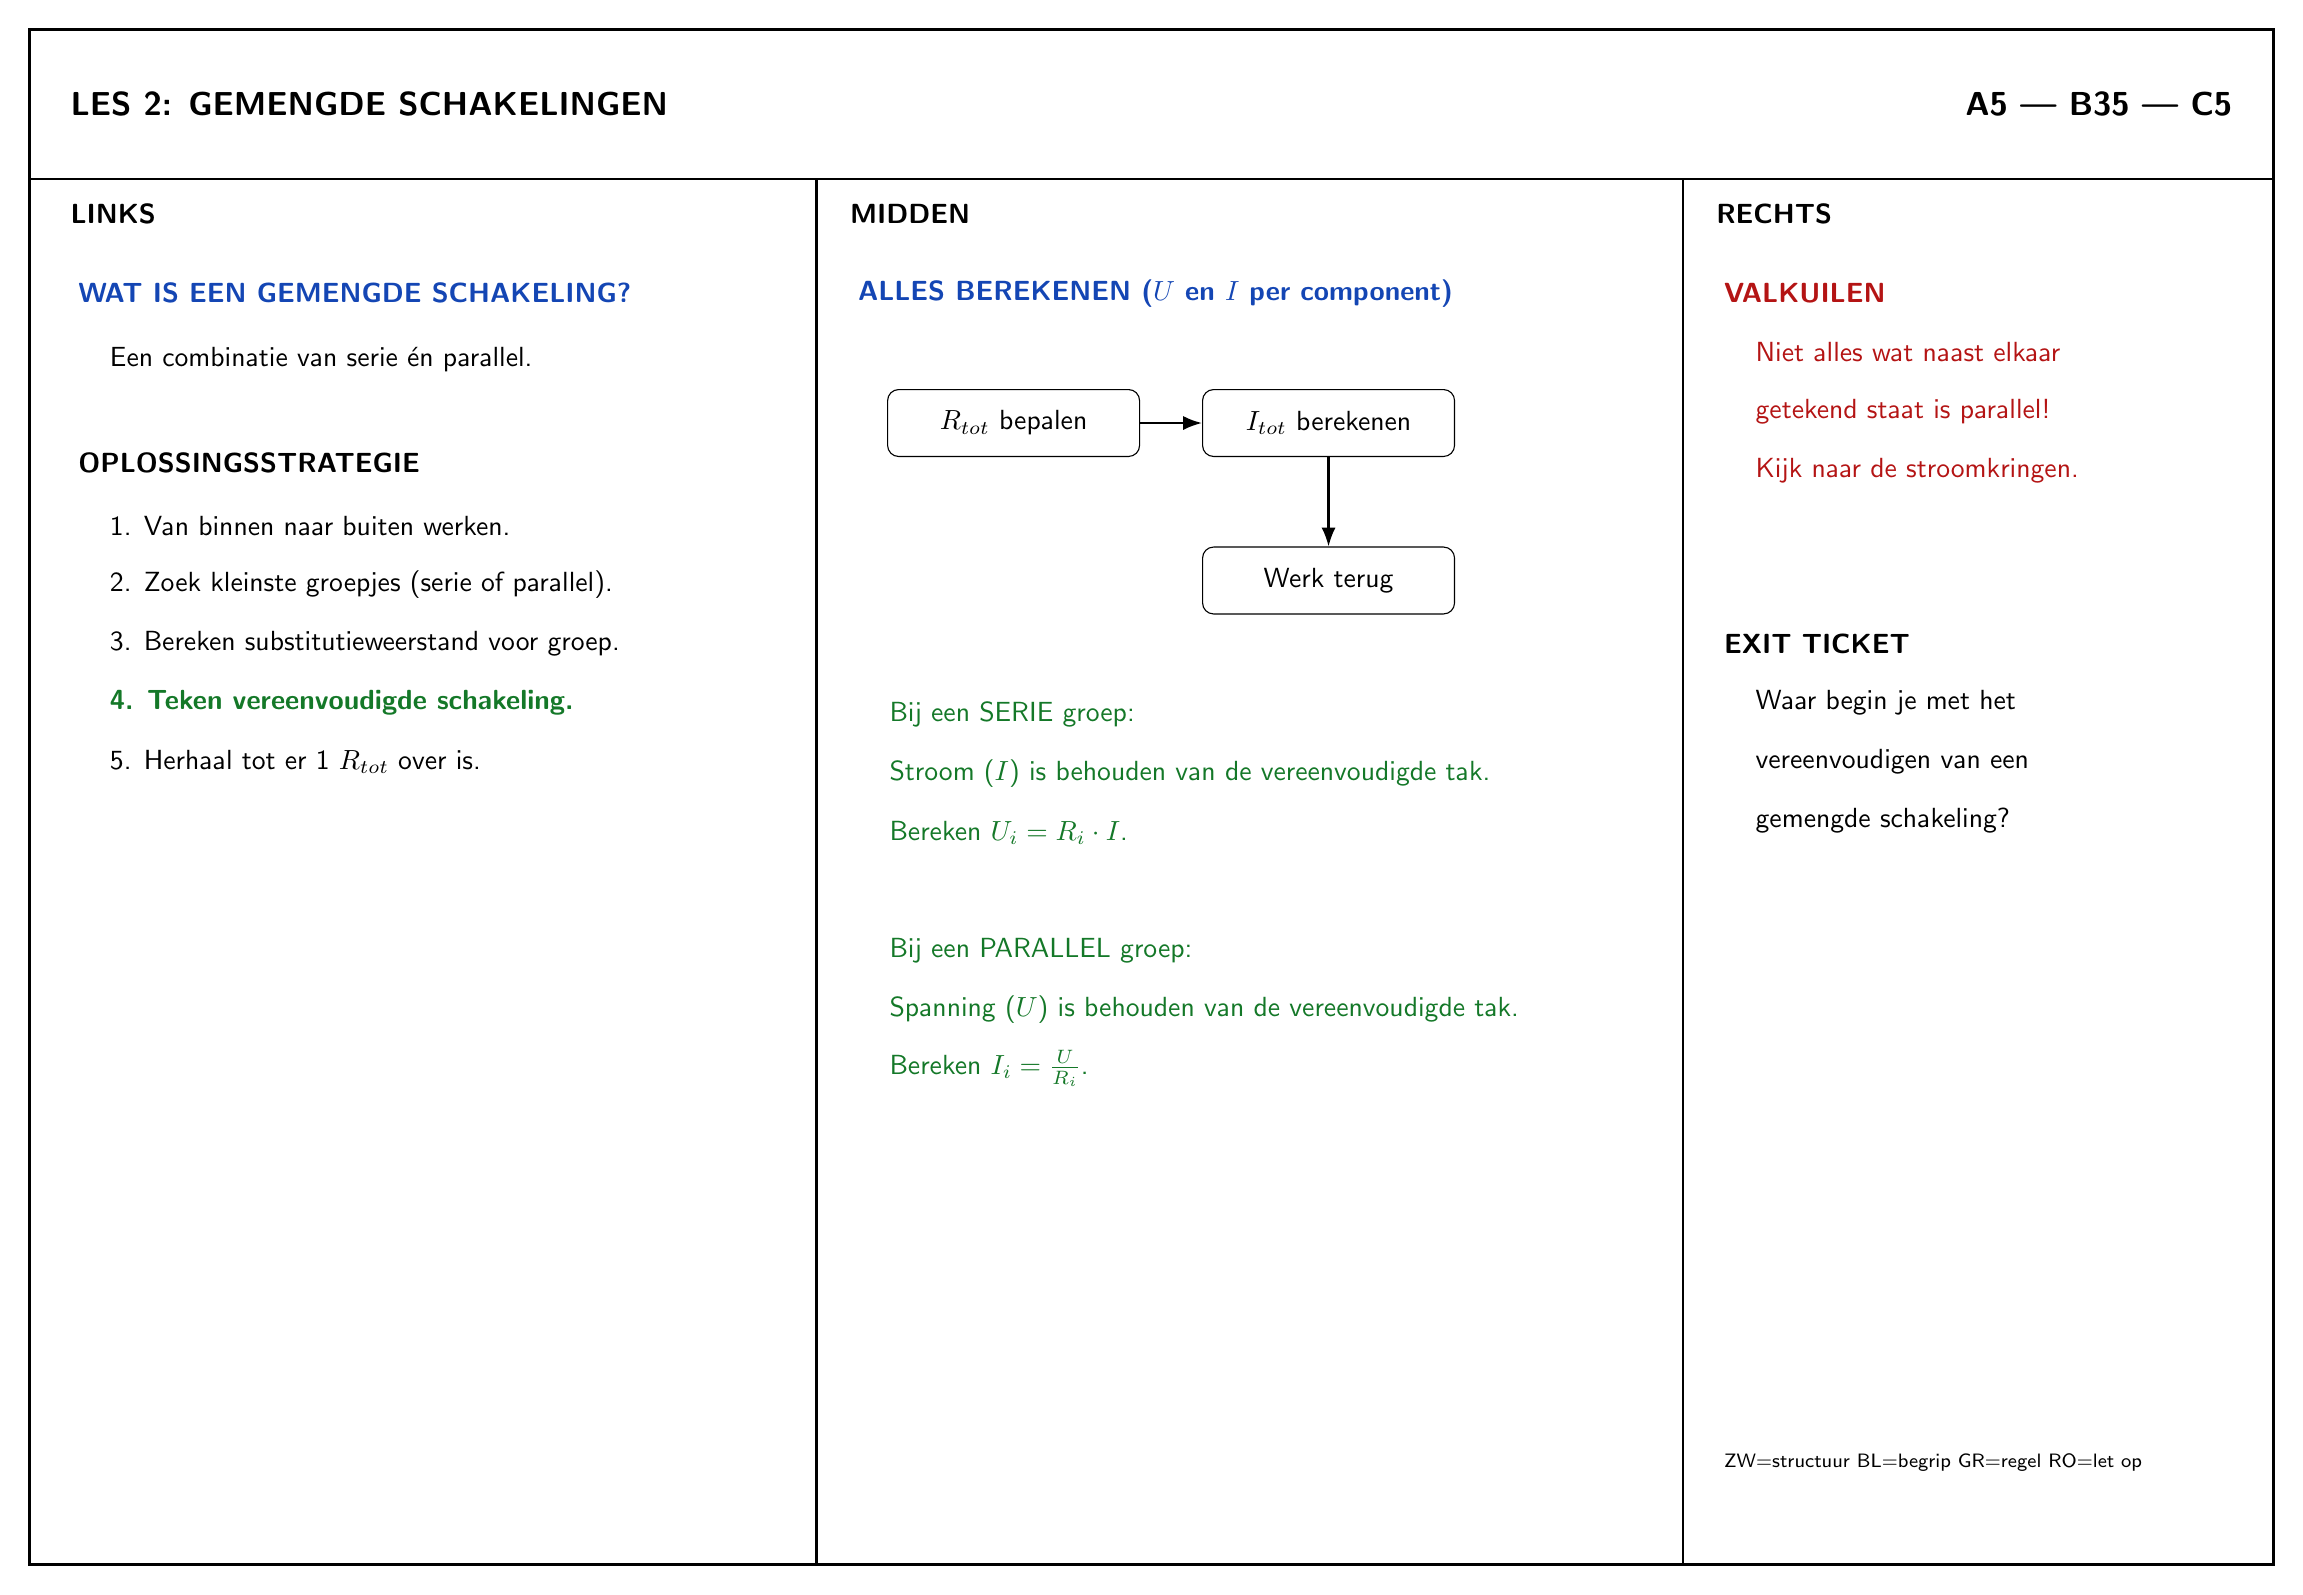
\begin{tikzpicture}[x=1cm,y=1cm]
  \draw[line width=1.2pt] (0,0) rectangle (28.5,19.5);
  \draw[line width=0.9pt] (0,17.6) -- (28.5,17.6);
  \node[anchor=west,font=\bfseries\large] at (0.4,18.55) {\ZW{LES 2: GEMENGDE SCHAKELINGEN}};
  \node[anchor=east,font=\bfseries\large] at (28.1,18.55) {\ZW{A5 | B35 | C5}};

  \draw[line width=0.9pt] (10.0,0) -- (10.0,17.6);
  \draw[line width=0.9pt] (21.0,0) -- (21.0,17.6);
  \node[anchor=west,font=\bfseries] at (0.4,17.15) {\ZW{LINKS}};
  \node[anchor=west,font=\bfseries] at (10.3,17.15) {\ZW{MIDDEN}};
  \node[anchor=west,font=\bfseries] at (21.3,17.15) {\ZW{RECHTS}};

  % left
  \node[anchor=west,font=\bfseries] at (0.5,16.15) {\BL{WAT IS EEN GEMENGDE SCHAKELING?}};
  \node[anchor=west] at (0.9,15.3) {\ZW{Een combinatie van serie én parallel.}};
  
  \node[anchor=west,font=\bfseries] at (0.5,14.0) {\ZW{OPLOSSINGSSTRATEGIE}};
  \node[anchor=west] at (0.9,13.2) {\ZW{1. Van binnen naar buiten werken.}};
  \node[anchor=west] at (0.9,12.45) {\ZW{2. Zoek kleinste groepjes (serie of parallel).}};
  \node[anchor=west] at (0.9,11.7) {\ZW{3. Bereken substitutieweerstand voor groep.}};
  \node[anchor=west,font=\bfseries] at (0.9,10.95) {\GR{4. Teken vereenvoudigde schakeling.}};
  \node[anchor=west] at (0.9,10.2) {\ZW{5. Herhaal tot er 1 $R_{tot}$ over is.}};

  % middle
  \node[anchor=west,font=\bfseries] at (10.4,16.15) {\BL{ALLES BEREKENEN ($U$ en $I$ per component)}};
  
  \node[draw,rounded corners,minimum width=3.2cm,minimum height=0.85cm] (l1) at (12.5,14.5) {\ZW{$R_{tot}$ bepalen}};
  \node[draw,rounded corners,minimum width=3.2cm,minimum height=0.85cm] (l2) at (16.5,14.5) {\ZW{$I_{tot}$ berekenen}};
  \node[draw,rounded corners,minimum width=3.2cm,minimum height=0.85cm] (l3) at (16.5,12.5) {\ZW{Werk terug}};
  \draw[-{Latex[length=2.4mm]},line width=0.8pt] (l1) -- (l2);
  \draw[-{Latex[length=2.4mm]},line width=0.8pt] (l2) -- (l3);

  \node[anchor=west] at (10.8,10.8) {\GR{Bij een SERIE groep:}};
  \node[anchor=west] at (10.8,10.05) {\GR{Stroom ($I$) is behouden van de vereenvoudigde tak.}};
  \node[anchor=west] at (10.8,9.3) {\GR{Bereken $U_i = R_i \cdot I$.}};
  
  \node[anchor=west] at (10.8,7.8) {\GR{Bij een PARALLEL groep:}};
  \node[anchor=west] at (10.8,7.05) {\GR{Spanning ($U$) is behouden van de vereenvoudigde tak.}};
  \node[anchor=west] at (10.8,6.3) {\GR{Bereken $I_i = \frac{U}{R_i}$.}};

  % right
  \node[anchor=west,font=\bfseries] at (21.4,16.15) {\RO{VALKUILEN}};
  \node[anchor=west] at (21.8,15.4) {\RO{Niet alles wat naast elkaar}};
  \node[anchor=west] at (21.8,14.65) {\RO{getekend staat is parallel!}};
  \node[anchor=west] at (21.8,13.9) {\RO{Kijk naar de stroomkringen.}};

  \node[anchor=west,font=\bfseries] at (21.4,11.7) {\ZW{EXIT TICKET}};
  \node[anchor=west] at (21.8,10.95) {\ZW{Waar begin je met het}};
  \node[anchor=west] at (21.8,10.2) {\ZW{vereenvoudigen van een}};
  \node[anchor=west] at (21.8,9.45) {\ZW{gemengde schakeling?}};

  \node[anchor=west,font=\scriptsize] at (21.4,1.3) {\ZW{ZW=structuur  BL=begrip  GR=regel  RO=let op}};
\end{tikzpicture}

\end{document}
